\documentclass[openany]{book}
% !TeX TXS-program:compile = txs:///pdflatex/[--shell-escape]
\usepackage{macros}
\usepackage{notes}

%% PICTURES DIRECTORY %%
\graphicspath{{C:/Users/Michael/Pictures/}}

%% REDEFINING CHAPTER FORMATTING %%
\newif\iftoc\titleformat{\chapter}[display]{\cabin}{}{2in}{
	\raggedleft
	\iftoc
	\vspace{2in}
	\else
	{\LARGE\textsc{Week}~{\cantarell\thechapter}} \\
	\fi
	\Huge\scshape\bfseries
}[\vspace{-20pt}\rule{\textwidth}{0.1pt}\vspace{0.0in}]
\titlespacing{\chapter}{0pt}{
	\iftoc
	-100pt+1in
	\else
	-130pt+1in
	\fi
}{0pt}

%% RENEW TITLE PAGE %%
\renewcommand{\mytitle}[2]{%
	\title{#1}
	\author{Michael Pham}
	\date{#2}
	\maketitle
	\newpage
	\mytoc
	\newpage
}

\begin{document}
\mytitle{EECS 127: Optimization Models in Engineering}{Fall 2024}

\chapter{Introduction}
\section{Lecture -- 8/29/2024}
\subsection{Motivating Examples}
To begin with, we will provide the following motivating examples:
\begin{example}[Oil Refinery]
	Suppose we have an oil refinery which produces jet fuel (at a profit of \$0.10/barrel) and gasoline (at a profit of \$0.20/barrel).
	
	From here, we have the following constraints: first, the oil refinery has a capacity of at most 10,000 barrels. Furthermore, it has a contract stating that it has to produce at least 1000 barrels of jet fuel and 2000 barrels of gasoline.
	
	Next, we know that the trucks has a capacity of 180,000 barrel-mile, with the jet fuel being 10 miles away, and gasoline being 30 miles.
	
	Then, we can model it as follows. First, let us denote $x_1$ to represent jet fuel, and $x_2$ to represent gasoline. Then, we have the following:
	\begin{align*}
		\max_{x_1, x_2} &\quad 0.1x_1 + 0.2x_2 \\
		\mathrm{s.t.} &\quad x_1 + x_2 \leq 10000 \\
		&\quad x_1 \geq 1000 \\
		&\quad x_2 \geq 2000 \\
		&\quad 10x_1 + 30x_2 \leq 180000
	\end{align*}

	And in this problem, we want to find the values of $x_1$ and $x_2$ which maximises the profit while staying within our constraints.
\end{example}

\begin{example}[Knapsack Problem]
	Suppose we have a set of $n$ items: $1, 2, \ldots, n$. Then, the item $i \in \brc{1, \ldots, n}$ has corresponding weight $w_i$ and value $v_i$.
	
	Furthermore, our bag has a weight capacity of at most $w$. Then, we want to select a set of items from our set such that the total value $v$ is maximised.
	
	To model this problem, we can first denote each item by a variable $x_i$, where $i \in \brc{1, \ldots, n}$. Next, we will have $x_i$ be an indicator variable such that $x_i = 1$ if the $i^{th}$ item is selected, and $0$ otherwise.
	
	The objective then is that we want to maximize $\sum_{i=1}^{n} v_i x_i$ while keeping to the constraints of $\sum_{i=1}^{n} w_i x_i \leq w$.
\end{example}

\subsection{Standard Form of Optimization}

\begin{defn}[Standard Form of Optimization]
	The standard form of optimization goes as follows:
	\begin{align*}
		\min_{f \in \RR^{n}} &\quad f_0(\vec{x}) \\
		\mathrm{s.t.} &\quad f_i(\vec x) \leq 0 \quad i \in \brc{1, \ldots, m} \\
		&\quad h_j(\vec x) = 0 \quad \forall j \in \brc{1, \ldots, p} 
	\end{align*}

	Here, we note that:
	\begin{itemize}
		\item $\vec x \in \RR^{n}$ is our optimization variable.
		\item $f_0(\vec x)$ is our objective function.
		\item $f_1, \ldots, f_m$ and $h_1, \ldots, h_p$ are functions $\RR^{n} \rightarrow \RR$.
		\item $f_i$ and $h_j$ are inequality and equality constraint functions respectively.
	\end{itemize}
\end{defn}

We note that if we are given a maximization problem, we can ``convert" it to a minimization problem by simply looking at $\min \pr{-f_0(\vec x)}$ instead when given $\max f_0(\vec x)$.

\begin{defn}[Feasible Solutions]
	We define $y \in \RR^{n}$ to be a feasible solution/point if it satisfies all of our constraints. Otherwise, it is an infeasible solution.
	
	We note that $y$ doesn't necessarily have to minimize our objective function.
\end{defn}

\begin{defn}[Feasible Sets]
	he feasible set -- denoted either by $\Omega$  or $X$ -- is the set of all feasible solutions. That is, we have
	\begin{equation*}
		X \coloneq \brc{\vec x \in \RR^{n} : f_1(\vec x) \leq 0, \ldots, f_m(\vec x) \leq 0}.
	\end{equation*}
\end{defn}

\begin{defn}[Global Minimum]
	We denote $x^{*}$ to be the ``global minimum" of our feasible set if $f_0(x^{*}) \leq f_0(x)$ for all $x \in X$.
\end{defn}

\begin{defn}[Local Minimum]
	A say that $x^{*}$ is a local minimum if there exists some neighbourhood around $x^{*}$ such that $f_0(x^{*}) \leq f_0(x)$ for all $x$ in our neighbourhood.
	
	We note here that if the radius of our ``ball" is $\pm \infty$, then we in fact have a global minimum.
\end{defn}
%\begin{enumerate}
%	\item First, we place all of our unknown variables into a vector. We often denote this vector by $x = \br{x_1, \ldots, x_n}^{\intercal}$
%	\item Next, we have the following: $\min_{x \in \RR^{n}} f_0(x)$ s.t. $f_1(x) \leq 0, \ldots, f_m(x) \leq 0$.
%\end{enumerate}

\chapter{Second Week Woes}
\section{Lecture -- 9/3/2024}
\subsection{Review}
Recall from the previous lecture that we denote $x^{*}$ to be the optimal solution, and $f_0(x^{*})$ to be the optimal objective value.

Then, the standard form would be the following: $\min_x f_0(x)$, such that $f_1(x) \leq 0, \ldots, f_m(x) \leq 0$.

Now, we had cases such as finding $\min x$; in this case, $x^{*} = -\inf$ and $f_0(x^{*}) = -\inf$. We say then that the optimal solution $x^{*}$ doesn't exist, and the function is unbounded from below.

In the case of $\min e^{x}$, we have that $x^{*} = -\inf$. However, note that $f_0(x^{*}) = 0$. Thus, while the optimal solution $x^{*}$ is not attainable, but the optimal objective value does exist.

And of course, the well-behaved case is when $x^{*}$ is attainable, and $f_0(x^{*})$ is fixed; they're both finite.

In the case where we have no feasible solution, recall that we call the problem is ``infeasible."

\begin{example}
	Suppose we have $\min x$, such that $x^{2} \leq -1$. We note that the optimization is infeasible, as we can't have $x^{2} \leq -1$.
	
	We say then that the optimal objective value, $f_0(x^{*})$, is equal to $+\infty$
\end{example}

Then, we have three cases for our optimal objective value:
\begin{enumerate}
	\item $+\infty$; in this case, it's infeasible.
	\item Finite; in this case, $x^{*}$ \textit{may} or may not be attainable.
	\item $-\infty$; in this case, it's unbounded from below.
\end{enumerate}

\subsection{Categories of Optimization Problems}
We say that optimization problems are either tractable or not-tractable.

\begin{defn}[Tractable vs Not-Tractable]
	A problem is ``tractable" is an algorithm exists to solve the problem. On the other hand, not-tractable problems are ones where an algorithm doesn't exist to solve the problem.
\end{defn}
\begin{warn}
	Note that not-tractable problems may have an algorithm to solve it, but it may not be fast enough.
\end{warn}

\begin{example}[Binary Decisions]
	Let us suppose we have to make $n$ decisions for a company to maximize their profits. For each decision, we have two options: yes or no.
	
	Then, we can map the $i^{th}$ decision to an indicator variable $x_i$, where $i \in \brc{1, \ldots, n}$.
	
	Then, we have that
	\begin{equation*}
		x_i = \begin{cases}
			+1 \text{ if yes.}\\ -1 \text{ if no.}
			\end{cases}
	\end{equation*}

	Then, we can write this as an optimization problem $\max f_0(x)$ (or $\min (-f_0(x))$), with the condition $x_i^{2} = 1$. This can be written as \begin{equation*}
		\begin{cases} x_i^{2}  - 1 \leq 0 \\ -x_i^{2} + 1 \leq 0 \end{cases}
	\end{equation*}
	
	Then, the number of feasible points is equal to $2^{n}$. Suppose we had $n = 500$; then, the number of evaluations of the objective function would be equal to $2^{500}$.
	
	Thus, the problem is not-tractable.
\end{example}

\begin{warn}
	Note that if problems can be solved within polynomial time, then it is tractable. Thus, in this class, we are looking at the class of ``convex optimization" problems.
\end{warn}

\begin{miscbox}{Interactable Functions and EECS 227B}
	Note that we have interactable problems; these are approximations. Suppose we wanted to minimize some function $\min f_0(x)$ that looks like the following:
%	include image lmfao; has a lot of local minimums

	To solve, it we can consider some smooth, underestimation of the actual function -- we call this $g_0(x)$. It is a much easier problem to look at than the original.
% include image of parabola lmfao
	
	The goal then is to make our approximation of the global minimum as close as possible to the real value.
\end{miscbox}

\subsection{Linear Al Jabr}
\begin{defn}[Space]
	A space is a collection of objects of a certain type.
\end{defn}

\begin{example}[$\RR^{n}$]
	For example, $\RR^{n}$ is a collection of vectors with $n$ elements.
\end{example}

We can also talk about things such as a space of matrices, polynomials, etc.
\begin{example}[$\mathscr{P}$]
	We can talk about the collection of polynomials with one variable, $a_0 + a_1t + \cdots + a_nt^{n}$.
\end{example}

\begin{defn}[Subspace]
	We define a subspace to be a non-empty set $V$ in our space $\RR^{n}$ with the following properties:
	\begin{itemize}
		\item The zero vector is contained in the subspace.
		\item For any two vectors $u, v \in V$, the linear combination $\alpha u + \beta v \in V$ as well.
	\end{itemize}
\end{defn}

\begin{example}[Examples in $\RR^{2}$]
	Suppose we are working in $\RR^{2}$. Then, consider the line $y = x$; we note that this is in fact a subspace of $\RR^{2}$ as it satisfies both conditions.
	% include image of y=x lmfao
	
	On the other hand, if our line no longer crosses the origin, it wouldn't be a subspace as $(0,0) \not\in V$.
	% include image of y = x + 1 lmfao
\end{example}

\begin{defn}[Span]
	We define the span of a set of vectors $S$ to be the set of linear combinations of vectors in $S$.
\end{defn}
\begin{example}
	Let us consider $m$ vectors: $x^{(1)}, x^{(2)}, \ldots, x^{(m)} \in \RR^{n}$.
	
	Then, we define $\vspan \pr{x^{(1)}, x^{(2)}, \ldots, x^{(m)}} = a_1x^{(1)} + \cdots + a_mx^{(m)}$. Note then that the span is in fact a subspace.
\end{example}

\begin{defn}[Basis]
	Let us consider a subspace $V$. Then, the basis is defined to be a linearly independent, spanning set of vectors $x_1, \ldots, x_n$ of $V$.
\end{defn}

\begin{defn}[Linear Independence]
	We say that a set of vectors $x_1, \ldots, x_m$ are linearly independent if only the trivial solution satisfies the following:
	\begin{equation*}
		a_1x_1 + \cdots + a_mx_m = 0
	\end{equation*}
	where $a_1, \ldots, a_m$ are scalars.
\end{defn}

\begin{example}
	Suppose we have the following:
	\begin{align*}
		x_1 &= \begin{bmatrix}
			1 \\ 1 \\ 1
		\end{bmatrix} \\
	x_2 &= \begin{bmatrix}
		1 \\ 2 \\ 3
	\end{bmatrix} \\
	x_3 &= \begin{bmatrix}
		-1 \\ 0 \\ 1
	\end{bmatrix}
	\end{align*} 

	Then, we define $V = \vspan(x_1, x_2, x_3)$. Note that this isn't linearly independent;  we note that $x_2 - 2x_1 = x_3$. Thus, they aren't a basis for $V$.
	
	Instead, if we considered $V = \vspan(x_1, x_2)$, then this would be linearly independent and thus is a basis.
	
	Similarly, if we considered $\vspan(x_1, x_3)$, this would also be a basis for $V$.
	
	Furthermore, we can see that $\dim V = 2$.
\end{example}

\begin{defn}[Affine Sets]
	A set is $X \subseteq \RR^{n}$ is an affine set if there exists a subspace $V$ of $\RR^{n}$ and a vector $x_0$ in $\RR^{n}$ such that $X = x^{0} + V$.
\end{defn}

\begin{example}
	Let us return to our example of $\RR^{2}$ with $y = x$. Then, let us consider the other example which wasn't a vector space (the shifted line); we note then that, in fact, it is an affine set. It's just a shifted version of our subspace.
\end{example}
\begin{warn}
	Clearly, affine sets may not go through the origin.
\end{warn}

\begin{defn}[Norm]
	We define the norm in $\RR^{n}$ to be a function $\norm{\cdot} : \RR^{n} \rightarrow \RR$ such that:
	\begin{enumerate}
		\item $\norm{x} \geq 0, \forall x \in \RR^{n}$.
		\item $\norm{x} = 0 \iff x = 0$.
		\item $\norm{x+y} \leq \norm x + \norm y, \forall x,y \in \RR^{n}$.
		\item $\norm{\alpha x} = \abs{\alpha} \norm x, \forall \alpha \in \RR, \forall x \in \RR^{n}$.
	\end{enumerate}
\end{defn}
\begin{example}[Examples of Norms]
	A norm on $\RR^{n}$ can be defined as the absolute value:
	\begin{equation*}
		\norm{x}_1 = \abs{x_1} + \abs{x_2} + \cdots + \abs{x_n}
	\end{equation*}

	This is called the $L_1$ norm.
	
	We can also define the following:
	\begin{equation*}
		\norm x_2 = \sqrt{x_1^{2} + x_2^{2} + \cdots + x_n^{2}}
	\end{equation*}

	This is called the $L_2$ norm.
	
	Furthermore, we have:
	\begin{equation*}
		\norm x_\infty = \max\brc{\abs{x_1}, \ldots, \abs{x_n}}
	\end{equation*}

	And the General $L_p$ Norm, where $1 \leq p < \infty$:
	\begin{equation*}
		\norm x_p = \pr{ \abs{x_1}^{p} + \cdots + \abs{x_n}^{p}}^{\frac{1}{p}}
	\end{equation*}

	Finally, the zero ``norm" is defined to simply be:
	\begin{align*}
		\norm x_0 &= \lim_{p \rightarrow 0} \pr{ \abs{x_1}^{p} + \cdots + \abs{x_n}^{p}}^{\frac{1}{p}} \\
		&= \card x \\
		&= \text{\# of non-zero elements of $x$}
	\end{align*}
\end{example}

\begin{defn}[Inner Products]
	We define the inner product to be a function on the space $X$ $\innerproduct{\cdot}{\cdot}: X \times X \rightarrow \RR$ such that:
	\begin{enumerate}
		\item $\innerproduct{x}{x} \geq 0, \forall x \in X$.
		\item $\innerproduct{x}{x} = 0 \iff x = 0$.
		\item $\innerproduct{x+y}{z} = \innerproduct{x}{z} + \innerproduct{y}{z}, \forall x,y,z \in X$.
		\item $\innerproduct{\alpha x}{y} = \alpha \innerproduct{x}{y}, \forall \alpha \in \RR, \forall x,y \in X$.
		\item $\innerproduct{x}{y} = \innerproduct{y}{x}, \forall x,y \in X$.
	\end{enumerate}
\end{defn}

\begin{example}
	Let us consider some inner product $\innerproduct{\cdot}{\cdot}$ on $\RR^{n}$ as follows:
	\begin{equation*}
		\innerproduct{x}{y} = \beta_1x_1y_1 + \cdots + \beta_nx_ny_n
	\end{equation*}

	where $\beta_1, \ldots, \beta_n > 0$. Note that if we let $\beta_1 = \cdots = \beta_n = 1$, then we get the ``standard" $\innerproduct{\cdot}{\cdot}$.
	
	Note we can also define $\innerproduct{x}{y} = \norm x_2 \norm y_2 \cos \theta$.
\end{example}

\section{Lecture -- 9/5/2024}
\subsection{Review}
Recall from the previous lecture that we discussed the notions of subspaces, affine sets, etc.

Furthermore, we denoted the inner product $\innerproduct{x}{y} = x_1y_1 + \cdots + x_ny_n = \norm{x}_2\norm{y}_2 \cos (\theta)$

And if $\innerproduct{x}{y} = 0$, this means that the two vectors are thus orthogonal.

\begin{example}[Applications of Linear Algebra]
	Given two published articles by two news outlets (e.g. CNN and Fox News), we want to see the similarity of the two articles.
	
	One way to do this is to create a simplified dictionary containing major key words, such as the following: \{president, tax, california, ...\}.
	
	Now, we define $x \in \RR^{n}$, where $x_i$ is the number of times the word $i$ appears in our first article. Similarly, we define $y \in \RR^{n}$, where $x_i$ is the number of times the word $i$ appears in the other article.
	
	Then, using the notion of inner product, we can first calculate $\cos \theta$; this gives us how similar these articles are. Namely, the closer $\cos \theta$ is to zero, the less similar the articles are to each other.
	
	On the other hand, the closer the value is to one, the more similar the articles are to each other. 
\end{example}

\section{Discussion -- 9/6/2024}
\subsection{Problem 1}
You have \$12,000 to invest at the beginning of the year, and three different funds from which to choose. The municipal bond fund has a 7\% yearly return, the local bank's CDs have an 8\% return, and a high-risk account has an expected 12\% return.

To minimize the risk, you decide not to invest more than \$2,000 in the high-risk account.

For tax reasons, you need to invest at least three times as much in the municipal bonds as in the bank CDs.
\begin{hw}
	Assuming the year-end yields are as expected, formulate the optimization problem in standard form.
\end{hw}
\begin{solution}
	We let $x_1, x_2, x_3$ to denote the amount of money we invest in the bond, CD, and high-risk account respectively.
	
	We want to maximize the following:
	\begin{equation*}
		\max_{x_1, x_2, x_3} 1.07x_1 + 1.08x_2 + 0.12x_3
	\end{equation*}

	Furthermore, we have the following conditions:
	\begin{align*}
		x_1 + x_2 + x_3 &\leq 12000 \\
		3x_2 &\leq x_1 \\
		x_3 &\leq 2000 \\
		0 &\leq x_1 \\
		0 &\leq x_2 \\
		0 &\leq x_3
	\end{align*}

	Putting this all together, we have the following:
	\begin{align*}
		\min_{x_1, x_2, x_3}&\quad -1.07x_1 - 1.08x_2 - 0.12x_3 \\
		\mathrm{s.t.}&\quad x_1 + x_2 + x_3 - 12000 \leq 0 \\
		&\quad -x_1 + 3x_2 \leq 0 \\
		&\quad x_3 - 2000 \leq 0 \\
		&\quad -x_1 \leq 0 \\
		&\quad -x_2 \leq 0 \\
		&\quad -x_3 \leq 0
	\end{align*}
\end{solution}

\begin{hw}
	If instead we were to invest exactly three times as much in the bonds as in the CDs, how would the problem change?
\end{hw}
\begin{solution}
	In this case, it would be the same other than the fact that we need to add in an extra condition $3x_1 - x_2 \leq 0$.
\end{solution}

\begin{warn}
	Note that we have the (hidden) constraint of the variables being non-negative...!
\end{warn}
\subsection{Problem 2}
A slalom skier must pass through $n$ parallel gates of known position $(x_i, y_i)$ and width $c_i$ with $i \in \brc{1, \ldots, n}$

\begin{hw}
	Write an optimization problem that minimizes the total length of the path in terms of the variables $\brc{(x_i, y_i, c_i)}_{i=0}^{n+1}$.
\end{hw}
\begin{solution}
	We can minimize the distance between each gate using the $L2$ norm. We denote $z_i$ to be the $y$ position of the skier at each time frame $i$:
	\begin{align*}
		\min_{z_0, \ldots, z_6} &\sum_{i=1}^{6} \norm{\begin{bmatrix}
				x_i \\ z_i
		\end{bmatrix} - \begin{bmatrix}
		x_{i-1} \\ z_{i-1}
	\end{bmatrix}}_2^{2}
%\\ = \min_{z_0, \ldots, z_6} &\sum_{i=1}^{6}  
	\end{align*}
	
	And we have the following conditions:
	\begin{align*}
		&y_i - \frac{c_i}{2} \leq z_i \leq y_i + \frac{c_i}{2} \\
		&z_0 = y_0 \\
		&z_6 = y_6
	\end{align*}
\end{solution}

\subsection{Problem 3}
\begin{hw}
	...
\end{hw}
\begin{solution}
	Let $x_1, x_2, x_3$ denote the number of servings for corn, milk, and bread respectively. Thus, we want to minimize:
	\begin{equation*}
		\min_{x_1, x_2, x_3} 0.15x_1 + 0.25x_2 + 0.05x_3
	\end{equation*}

	And we have the following conditions:
	\begin{align*}
		&x_1 + x_2 + x_3 \leq 10 \\
		&2000 \leq 70x_1 + 121x_2 + 65x_3 \leq 2250 \\
		&5000 \leq 107x_1 + 500x_2 + 0x_3 \leq 10000 \\
		&45x_1 + 40x_2 + 60x_3 \leq 1000 \\
		& x_1, x_2, x_3 \geq 0
	\end{align*}
\end{solution}

\subsection{Problem 4}
\begin{hw}
	...
\end{hw}
\begin{solution}
	For each intersection $j$, let $q_i$ represent the flow of traffic on each road segment coming in/out of our intersection.
	
	Then, $q_i < 0$ denotes traffic going out, and $q_i > 0$ indicates traffic flowing in.
	
	Then, for each intersection $j$, we can denote $v_j$ to denote a vector as follows:
	\begin{equation*}
		v_j = \begin{bmatrix}
			q_1 \\ \vdots \\ q_i
		\end{bmatrix}
	\end{equation*}

	Then, we can use a matrix with $j$ rows and $i$ columns such that each entry in our matrix determines whether there is flowing in or out of traffic due to a road $q_i$ for the corresponding $j^{th}$ intersection.
\end{solution}

\begin{hw}
	...
\end{hw}
\begin{solution}
	To stay close to the historical data, we can use the $L2$ norm such that
\end{solution}

\chapter{Third Week}
\section{Lecture -- 9/10/2024}
\subsection{Projection Review}
\begin{example}[Formula for Projection on $d$-dimension Subspaces]
	Let $S$ be a $d$ dimensional subspace. Define a basis $x_1, \ldots, x_d$ for $S$. Then, this means that $S = \vspan\pr{x_1, \ldots, x_d}$.
	
	Then, we want to project some vector $x \in \RR^{n}$ onto the subspace $S$. Now, note that since the projection $x^{*} \in S$, it can be written as a linear combination of the basis vectors of $S$.
	
	That is, we can write $x^{*}$ as such:
	\begin{equation*}
		x^{*} = \alpha_1x_1 + \cdots + \alpha_dx_d
	\end{equation*}

	Recall from last time that $\ang{x - x^{*}, y} = 0$, for all $y \in S$.
	
	Then, let us pick $y$ to be $x_j$ for $j \in \brc{1, \ldots, d}$. Then, we have:
	\begin{align*}
		\ang{x - x^{*}, y} &= \ang{x - \sum_{i=1}^{d} \alpha_i x_i, x_j} \\
		&= 0 \quad\text{for $j = 1, \ldots, d$} \\
		\ang{\sum_{i=1}^{d} \alpha_i x_i, x_j} &= \ang{x, x_j} \\
		\sum_{i=1}^{d}\alpha_i \ang{x_i, x_j} &= \ang{x, x_j}
	\end{align*}
	
	From here, we can expand the summation out for each $j$ to get the following:
	\begin{equation*}
		\begin{cases}
			\alpha_1\ang{x_1, x_1} + \cdots + \alpha_d\ang{x_d, x_1} = \ang{x, x_1} \\
			\vdots \\
			\alpha_1\ang{x_1, x_d} + \cdots + \alpha_d\ang{x_d, x_d} = \ang{x, x_d}.
		\end{cases}
	\end{equation*}

	Now, we see that we have $d$ equations with $d$ unknown variables $\alpha_1, \ldots, \alpha_d$. Then, if $x_1, \ldots, x_d$ is orthonormal, then recall that $\ang{x_i, x_j} = 0$ for $i \neq j$.
	
	Thus, in fact, we have the following:
	\begin{align*}
		a_j \ang{x_j, x_j} &= \ang{x, x_j} \quad \text{for $j = 1, \ldots, d$} \\
		a_j &= \ang{x, x_j}
	\end{align*}

	Now, going back to the projection, we call that $\prod_{S}^{}(x) = x^{*} = \alpha v = \ang{x, x_1}x_1 + \cdots + \ang{x, x_2}x_2$.
\end{example}

\subsection{Hyperplanes and Half-Spaces}
\subsubsection{Hyperplanes}
\begin{defn}[Hyperplane]
	Let us denote a hyperplane as $H$. Then, this is an $n-1$ dimensional affine set which can be written as a set of vectors $z \in \RR^{n}$ such that $a^{\intercal}z = b$, where $a$ is non-zero.
	
	That is, we have:
	\begin{equation*}
		H = \brc{z \in \RR^{n} : a^{\intercal} z = b}.
	\end{equation*}
\end{defn}

\begin{example}[Hyperplane in $\RR^{3}$]
	In $\RR^{3}$, the hyperplane will be two dimensional. Now, let us pick two vectors $z_1, z_2 \in H$ such that $a^{\intercal} z_1 = b$ and $a^{\intercal} z_2 = b$.
	
	Subtracting the two equations, we then get $a^{\intercal}\pr{z_1 - z_2} = 0$. Thus, we conclude that $a \perp \pr{z_1 - z_2}$ (that is, $a$ is orthogonal to $z_1 - z_2$).
	
	$a$ has a special name: it is the ``normal vector" of our hyperplane.
\end{example}
\begin{hw}
	Find a formula for the projection onto $H$
\end{hw}
\begin{solution}
	...
\end{solution}

\subsubsection{Half-Spaces}
\begin{defn}[Half-Spaces]
	We say that a hyperplane $H$ divides our space into two regions:
	\begin{enumerate}
		\item $H_- = \brc{x : a^{\intercal}x \leq b}$
		\item $H_+ = \brc{x : a^{\intercal} \geq b}$.
	\end{enumerate}
\end{defn}

\subsection{Unconstrained Optimization}
This idea of unconstrained optimization $\min_{x \in \RR^{n}} f(x)$ shows up quite often. For example, it appears in least-squares.

Before we explore this notion, we must first review certain terms.

\subsubsection{Gradient}
\begin{defn}[Gradient]
	We define the gradient as follows:
	\begin{equation*}
		\nabla f(x) = \begin{bmatrix}
			\frac{\partial f(x)}{\partial x_1} \\
			\vdots \\
			\frac{\partial f(x)}{\partial x_n}
		\end{bmatrix}
	\end{equation*}

	We note that if $n = 1$, then it's the same as the derivative.
\end{defn}

\begin{example}
	Suppose we have $f(x) = \sin x_1 + 4x_1x_2 + x_2^{2}$. Then, the gradient is:
	\begin{equation*}
		\nabla f(x) = \begin{bmatrix}
			\cos x_1 + 4x_2 \\
			4x_1 + 2x_2
		\end{bmatrix}
	\end{equation*}
\end{example}

\begin{example}
	Suppose we have $f(x) = \norm{x}_2^{2}$. Then, we see that $f(x) = x_1^{2} + \cdots + x_n^{2}$. Then, we see that the gradient is simply:
	\begin{align*}
		\nabla f(x) &= \begin{bmatrix}
			2x_1 \\
			\vdots \\
			2x_n
		\end{bmatrix} \\
		&= 2x
	\end{align*}
\end{example}

\begin{example}
	If $f(x) = \norm{x}_2$, we note that the gradient doesn't exist if $x = 0$. And we claim that if $x \neq 0$, we have:
	\begin{equation*}
		\nabla f = \frac{x}{\norm{x}}.
	\end{equation*}
\end{example}

\subsubsection{Types of Functions}
\begin{defn}[Linear Functions]
	We say that $f: \RR^{n} \rightarrow \RR$ is linear if $f(\alpha x + \beta y) = \alpha f(x) + \beta f(y)$, for all $\alpha, \beta \in \RR$ and $x, y \in \RR^{n}$.
\end{defn}

\begin{prop}
	If $f(x)$ is a linear function, we claim that there exists a vector $a \in \RR^{n}$ such that $f(x) = a^{\intercal x}$.
\end{prop}

\begin{defn}[Affine Functions]
	We say that $f : \RR^{n} \rightarrow \RR$ is an affine function if $f(x) - f(0)$ is a linear function.
\end{defn}

\begin{prop}
	We thus claim that there exists $a \in \RR^{n}$ and $b \in \RR$ such that $f(x) = a^{\intercal} x + b$, where $b = f(0)$.
\end{prop}

\begin{prop}
	We note that if $f$ is an affine function, then $\nabla f(x) = a$.
\end{prop}

\subsubsection{Chain Rule for Gradient}
\begin{thm}
	Consider $f : \RR^{m} \rightarrow \RR$ and $g : \RR^{n} \rightarrow \RR^{m}$.
	
	Then, we define $\varphi (x) = f(g(x))$. The gradient $\nabla \varphi(x)$ will thus be:
	\begin{equation*}
		\nabla \varphi(x) = \begin{bmatrix}
			\nabla g_1(x) & \cdots & \nabla g_m(x)
		\end{bmatrix} \times \nabla f(z) \big|_{z = g(x)}
	\end{equation*}
	
%	Then, we have
%	\begin{equation*}
%		g(x) = \begin{bmatrix}
%			g_1(x) \\ \vdots \\ g_m(x)
%		\end{bmatrix}
%	\end{equation*}
\end{thm}

\begin{example}
	Let us look at:
	\begin{equation*}
		\begin{bmatrix}
			x_1 \\ x_2
		\end{bmatrix} \rightarrow 
		\begin{bmatrix}
			2x_1 + 5x_2 + 1 \\ -x_1 + 5x_2 - 5
		\end{bmatrix}
	\end{equation*}

	Then, $f(x) = f(x_1, x_2)$, and $\varphi = f(2x_1 + 5x_2 + 1, -x_1 + 5x_2 - 5)$. Then, we have the following:
	\begin{align*}
		\nabla \varphi(x) &= \begin{bmatrix}
			\nabla (2x_1 + 5x_2 + 1) & \nabla(-x_1 + 5x_2 - 5)
		\end{bmatrix} \times \nabla f(z) \\
		&= \begin{bmatrix}
			2 & -1 \\ 5 & 5
		\end{bmatrix} \times \nabla f(z)\big|_{z=g(x)}
	\end{align*}
\end{example}

\subsubsection{Taylor Series}
Given a function $f : \RR^{n} \rightarrow \RR$ which is differentiable, at a point $x_0 \in \RR^{m}$, we can approximate the function with an affine function in a neighbourhood of $x_0$.

Recall that $f(x) = f(x_0) + \nabla f_{(x_0)}^{\intercal}(x - x_0) + \zeta(x)$. And we note that
\begin{equation*}
	\lim_{x \rightarrow x_0} \frac{\zeta(x)}{\norm{x-x_0}} = 0
\end{equation*}

That is, $f(x) \approx f(x_0) + \nabla f_{(x_0)}^{\intercal}(x- x_0)$. Thus, we see that it's an affine function in $x$.

\begin{thm}
	If $x^{*}$ is a local minimization of $\min_{x \in \RR^{n}} f(x)$, where $f(x)$ is differentiable at $x^{*}$, then the gradient $\nabla f(x^{*}) = 0$.
\end{thm}
\begin{proof}
	Since $x^{*}$ is a local minimum, we note that $\exists r > 0$ such that $f(x^{*}) \leq f(x)$, $\forall x : \norm{x - x^{*}} \leq r$. 
	
	Then, we see that $x^{*} + ty$ will be inside our neighbourhood for sufficiently small $t$. Then, we have:
	\begin{align*}
		f(x^{*} + ty) &\geq f(x^{*}) \\
		0 &\leq \frac{f(x^{*} + ty) - f(x^{*})}{t} \quad t > 0, \text{$\forall t$ : small} \\
		0 &\leq \lim_{t \rightarrow 0^{+}} \frac{f(x^{*} + ty) - f(x^{*})}{t} \\
		&= \frac{\partial f(x^{*} + ty)}{\partial t} \big|_{t = 0} \\
		&= \frac{\partial f (x_1^{*} + ty_1, \ldots, x_n^{*} + ty_n)}{\partial t} \big|{t = 0} \\
		&= \sum_{i=1}^{n} \frac{\partial(x_i^{*} + ty_i)}{\partial t} \times \frac{\partial f(z)}{\partial x_i} \big|_{z = x^{*} + ty\text{ with $t = 0$}} \\
		&= \sum_{i=1}^{n} y_i \frac{\partial f(x^{*})}{\partial x_i} \\
		&= y^{\intercal} \nabla f(x^{*})
	\end{align*}

	Now, since $y$ can be some arbitrary value that eventually gets scaled to be within our neighbourhood, let us set $y = -\nabla f(x^{*})$. Then, we have:
	\begin{align*}
		0 &\leq -\nabla f(x^{*})^{\intercal} \nabla f(x^{*}) \\
		&= - \norm{\nabla f (x^{*})}^{2} \\
		\implies & \norm{\nabla f(x^{*})} = 0 \implies \nabla f(x^{*}) = 0
	\end{align*}
\end{proof}

\subsubsection{Least-Squares}
Let us consider $\min_{x \in \RR^{n}} f(x)$, where $f(x) = \norm{Ax - b}$, where $A$ is an $n \times n$ matrix, and $b \in \RR^{m}$.

\begin{example}[Expressing Systems of Equations with Matrices]
	Suppose we ahve $3$ equations and $2$ unknowns:
	\begin{align*}
		x_1 - x_2 &= 1 \\
		2x_1 + 5x_2 &= -1 \\
		-0.5x_1 + 3.5x_2 &= 10
	\end{align*}

	We can express this as a matrix as follows:
	\begin{equation*}
		\begin{bmatrix}
			1 & -1 \\
			2 & 5 \\
			-0.5 & 3.5
		\end{bmatrix}
		\begin{bmatrix}
			x_1 \\ x_2
		\end{bmatrix} =
		\begin{bmatrix}
			1 \\ -1 \\ 10
		\end{bmatrix}
	\end{equation*}
\end{example}

\begin{example}[Fitting Power Law to Data]
	Suppose we have some system as follows:
	\begin{center}
		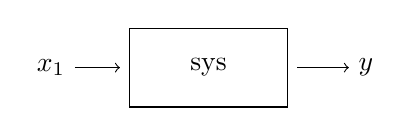
\begin{tikzpicture}
			\node (x1) at (-2, 0) {$x_1$};
			\node (sys-1) at (-1, 0) {};
			\node (sys) at (0, 0) {sys};
			\node (sys+1) at (1, 0) {};
			\node (y) at (2, 0) {$y$};
			\draw (-1, 0.5) rectangle (1, -0.5);
			\draw[->] (x1) -- (sys-1);
			\draw[->] (sys+1) -- (y);
		\end{tikzpicture}
	\end{center}

	Now, we say that $y = \alpha x_1^{a_1} \cdots x_n^{a_n}$. We have $\alpha, a_1, \ldots, a_n$ unknown variables.
	
	Now, we have the following inputs to outputs:
	\begin{equation*}
		\begin{cases}
			x_1 \\ \vdots \\ x_m
		\end{cases}
		\rightarrow
		\begin{cases}
			y_1 \\ \vdots \\ y_m
		\end{cases}
	\end{equation*}

	Now, we consider $\log (y) = \log(\alpha) + a_1\log x_1 + \cdot + a_n \log x_n$. Then, we have:
	\begin{equation*}
		\begin{bmatrix}
			1 & \tilde{x}_1^{(1)} & \cdots & \tilde{x}_n^{(1)} \\
			\vdots & &  & \\
			1 & \tilde{x}_1^{(m)} & \cdots & \tilde{x}_n^{(m)}
	 	\end{bmatrix}
 		\begin{bmatrix}
 			\tilde{\alpha} \\
 			a_1 \\
 			\vdots \\
 			a_n
 		\end{bmatrix}
	\end{equation*}
\end{example}

\section{Lecture -- 9/12/2024}
\subsection{Examples}
\begin{example}[CAT Example]
	To begin with, with can imagine an array of voxels. We denote $x_i$ to be the density of the voxel $i$.
	
	Then, we have the following equation:
	\begin{equation*}
		I_1 = I_0 e^{-a_1x_1 - \cdots - a_nx_n}.
	\end{equation*}
	
	Rearranging this, we get:
	\begin{align*}
		e^{-a_1x_1 - \cdots - a_nx_n} &= \frac{I_0}{I_1} \\
		-a_1x_1 - \cdots - a_nx_n &= \log\pr{\frac{I_0}{I_1}}
	\end{align*}
	
	Now, recall that each $a_i$ denotes the beam $i$. Then, we have: ...
\end{example}

\subsection{Rank and Null Space}
Consider $Ax = y$, where $A, y$ are known, but $x$ unknown. $A$ is of dimension $m \times n$, $x$ is $n \times 1$, and $y$ is $m \times 1$.

Now, the solution set is defined as:
\begin{equation*}
	S = \brc{x \in \RR^{n} : Ax = y}.
\end{equation*}

Before we proceed, we need two notions:
\begin{itemize}
	\item The range of $A$ -- denoted by $R(A)$ -- is the set of $Ax$ such that $x \in \RR^{n}$. That is,
	\begin{equation*}
		R(A) = \brc{Ax : x \in \RR^{n}}.
	\end{equation*}
	\begin{itemize}
		\item Furthermore, we say that the dimension of $R(A)$ to be denoted by $\rank (A)$.
	\end{itemize}
	\item The null-space $N(A)$ is defined as:
	\begin{equation*}
		N(A) = \brc{x \in \RR^{n} : Ax = 0}.
	\end{equation*}
\end{itemize}

\begin{thm}
	The rank of a matrix $A$ is equal to the number of linearly independent columns of $A$.
\end{thm}
\begin{cor}
	The rank of a matrix $A$ is equal to the number of linearly independent rows of $A$.
\end{cor}

Thus, we have the following line inequalities:
\begin{align*}
	\rank(A) &\leq \text{maximum number of rows or columns} \\
	0 &\leq \rank(A) \leq \min\pr{m, n}
\end{align*}

\begin{cor}
	If $\rank (A) = 0$, then $A = 0$.
\end{cor}

\begin{thm}[Fundamental Theorem of Linear Algebra]
	We have the following two statements:
	\begin{enumerate}
		\item $N(A) \perp R(A^{\intercal})$
		\item $N(A) \oplus R(A^{\intercal}) = \RR^{n}$.
		\item $\dim N(A) + \rank (A) = n$.
	\end{enumerate}
\end{thm}
\begin{proof}
	First, we will show that $N(A) \perp R(A^{\intercal})$.
	\begin{innerproof}
		To begin with, let us take $v \in N(A)$. Then, by definition, we have that $Av = 0$. 
		
		Now, let us take some $w \in R(A^{\intercal})$. Then, we note that there exists some $u \in \RR^{m}$ such that $A^{\intercal}u = w$.
		
		Then, we observe that $\ang{v,w} = v^{\intercal}w = v^{\intercal}A^{\intercal}u = (Av)^{\intercal}u = 0$.
	\end{innerproof}

	Next, we prove the second statement. It says then that for any $h \in \RR^{n}$, there exists some $v \in N(A)$ and $w \in \RR(A^{\intercal})$ such that $h = v + w$.
	\begin{innerproof}
	...
	\end{innerproof}
\end{proof}

Now, let us go back to the equation $Ax = y$. We have a solution in each of the three cases:
\begin{enumerate}
	\item $y \in R(A)$.
	\item $y$ is in the span of the columns of $A$.
	\item $\rank (A) = \rank \br{A y}$.
\end{enumerate}

\begin{example}
	First, let us pick an arbitrary solution $\bar x$: $A \bar x = y$. Then, we observe that $Ax = y$ reduces to $A(x - \bar x) = 0$.
	
	Let $z = x - \bar x$. Then, we observe that $z \in N(A)$. Then, we observe that every solution $x$ is equal to $\bar x + z$; i.e. it's the sum of $\bar x$ and a vector in the null space of $A$.
\end{example}

Thus, in fact, we can write $S = \bar x + N(A)$.

\begin{rmk}
	In fact, we note that the solution set $S$ is actually an affine set. Though if the null space of $N(A)$ is zero, we note then that $S$ has only one element; the solution is unique.
\end{rmk}

Now, in the case where we have infinitely many solutions, the question then arises: how do we pick the best one?

In this case, we want $\min_{x \in \RR^{n}} \norm{x}$, such that $Ax = y$.

Then, $u^{*}$ is defined to be the projection of $0$ onto $S$. Then, we project $0$ onto $S = \bar x + N(A)$ (recall that $S$ is an affine set!). Then, since $x^{*} \in S$, we have $x^{*} - \bar x \in N(A)$.

Thus, we have $\ang{x^{*}, x^{*} - \bar x} = 0$, for all $x \in S$. Thus, we conclude that $x^{*}$ is orthogonal to the null space $N(A)$. And therefore, we note that $x^{*} \in R(A^{\intercal})$.
\end{document}